
\documentclass{beamer}
\usetheme{metropolis} % Use the metropolis theme



% Add tikz and pgfplots packages
\usepackage{tikz, pgfplots}
\usetikzlibrary{positioning}

% For clicking references
\usepackage{hyperref}

% For better referencing
\usepackage{cleveref}

\usepackage{graphicx}

% Define custom pastel colors
\definecolor{pastelRed}{RGB}{255, 105, 97}   % A soft pastel red
\definecolor{pastelBlue}{RGB}{119, 158, 203} % A muted pastel blue
\definecolor{pastelYellow}{RGB}{255, 223, 0} % A gentle pastel yellow
\definecolor{lightGray}{RGB}{211, 211, 211}  % A light gray for subtitles and less emphasized text

% Apply the custom colors
\setbeamercolor{palette primary}{bg=black, fg=white}
\setbeamercolor{palette secondary}{bg=lightGray, fg=black}
\setbeamercolor{palette tertiary}{bg=black, fg=white}
\setbeamercolor{titlelike}{parent=palette primary, fg=black}
\setbeamercolor{subtitle}{fg=lightGray}
\setbeamercolor{structure}{fg=black} % For itemize, enumerate, etc

% Change color of normal text
\setbeamercolor{normal text}{fg=black, bg=white}

% Set the color of the table of contents
\setbeamercolor{section in toc}{fg=black} % Section titles in TOC
\setbeamercolor{subsection in toc}{fg=black} % Subsection titles in TOC

% Set block colors
\setbeamercolor{block title}{use=structure,fg=white,bg=pastelRed}
\setbeamercolor{block body}{fg=black,bg=white}



% Title Page Info
\title{Inclusion-Exclusion}
\subtitle{Spørgsmål 2 fra Exam Questions}
\author{Kevin Vinther}
\date{\today}

\begin{document}

% Title Page
\begin{frame}
    \titlepage
\end{frame}

% Table of Contents
\begin{frame}[allowframebreaks]
    \frametitle{Table of Contents}
    \tableofcontents
\end{frame}

\section{The Inclusion-Exclusion Principle}

\begin{frame}{Sum \& Subtraction Rule}
   \begin{itemize}
       \item Tilbagekald sum-reglen
       \item Hvis to tasks $n_1$ og $n_2$ kan gøres på hver sin måde, og de ikke har nogen af disse måder tilfælles, så er der $n_1 + n_2$ måder at gøre dette på
       \item Subtraction-rule udvider på dette
       \item Den tillader, at tasksne har noget tilfælles. Så er der $n_1 + n_2 - n_3$ måder at gøre det på, hvor $n_3$ er det fælles antal af måder man kan gøre $n_1$ og $n_2$ på.
   \end{itemize} 
\end{frame}

\begin{frame}{Begyndelsen}
   \begin{itemize}
       \item Før vi kommer til inclusion exclusion, tager vi et yderligere kig på subtraction rule, men for sæt:
       \item $|A \cup B| = |A| + |B| - |A \cap B|$
   \end{itemize} 
\end{frame}


\begin{frame}{Eksempel 1}
\begin{columns}
\begin{column}{0.5 \textwidth}
   \begin{itemize}
       \item<1-> I en klasse studerer alle elever enten datalogi eller matematik, eller begge. Der er i alt 25 datalogi studerende, og 13 matematikstuderende. Derudover er der 8 der studerer både matematik og datalogi. Hvor mange studerende er der i alt? 
       \item<2-> $|A \cup B| = |A| + |B| - |A \cap B| = 25 + 13 - 8 = 30$
   \end{itemize} 
\end{column}
\begin{column}{0.5 \textwidth}
\pause
   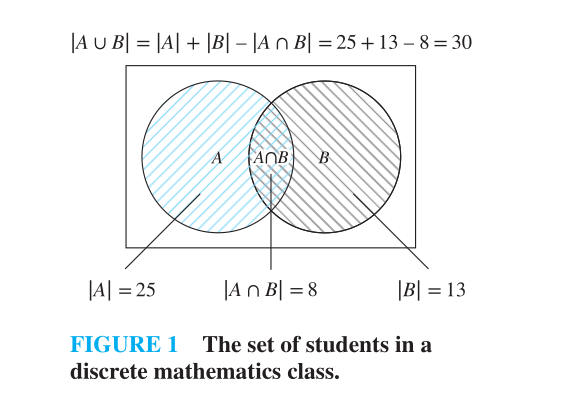
\includegraphics[scale=0.36]{81fig1.png} 
\end{column}
\end{columns}
\end{frame}

\begin{frame}{Eksempel 2}
   \begin{itemize}
       \item<1-> Der kommer mange eksempler, da jeg tænker Jørgen vil have du kan (næsten) alle.
       \item<1-> Hvor mange positive heltal, som ikke overstiger 100, er delelig med 7 eller 11?
       \item<2-> Hvis vi siger at A er et sæt med tal der er delelige med 7 under 1000
       \item<2-> Og B med 11 under 1000
       \item<2-> Så er $|A \cup B|$ delelige med enten 7 eller 11 under 1000.
       \item<3-> Der er $\lfloor \frac{1000}{7} \rfloor$ tal der er delelige med 7 under 1000, og $\lfloor \frac{1000}{11} \rfloor$ tal der er delelige med 11. 
       \item<3-> Dermed er der $\lfloor\frac{1000}{7\cdot11}\rfloor$ tal der er delelige med \textbf{både} 7 og 11. Så svaret er:
       \item<4-> $\lfloor \frac{1000}{7} \rfloor + \lfloor \frac{1000}{11} \rfloor - \lfloor \frac{1000}{11\cdot7} \rfloor = 142+90-12=220 $
   \end{itemize} 
\end{frame}

\begin{frame}{Eksempel 2 Figur}
   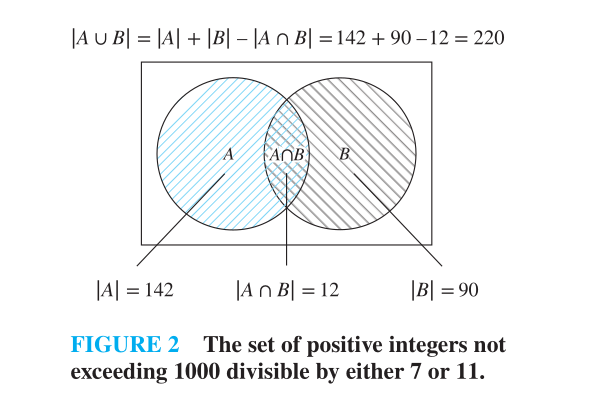
\includegraphics[scale=0.8]{81fig2.png} 
\end{frame}

\begin{frame}{Inclusion-Exclusion for 3 sæt}
   \begin{itemize}
       \item<1-> Hvad gør vi så når vi skal bruge mere end to sæt? 
       \item<1-> Antag at vi vil finde kardinaliteten af fællesmængden af tre sæt $|A \cup B \cup C|$.
       \item<1-> Vil det være nok bare at sige $|A| + |B| + |C| - |A \cap B \cap C|$
       \item<2-> \textbf{Nej}. Hvorfor ikke?
       \item<3-> $|A| + |B| + |C|$ overtæller ikke bare fællesmængden af alle sæt, men også:
       \item<3-> Et element der kun er i et af de tre sæt bliver talt én gang. Et element der er i to sæt bliver talt to gange, og et element der er i tre sæt blive talt tre gange. 
   \end{itemize} 
\end{frame}

\begin{frame}{Antal af elementer i sæt}
\begin{center}
    
    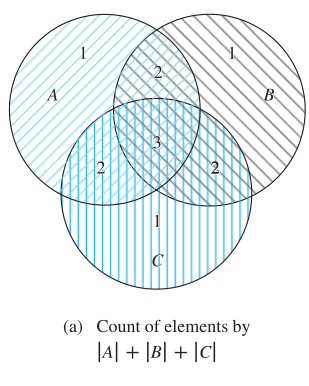
\includegraphics[scale=0.8]{81fig3a.png}
\end{center}
\end{frame}

\begin{frame}{3 sæt contd. }
   \begin{itemize}
       \item<1-> Så, siden der bliver talt for mange gange, skal vi fjerne overtælningerne. Hvordan gør vi det? 
       \item<2-> $|A|+|B|+|C| - |A \cup B| - |B \cup C| - |A \cup C|$
       \item<2-> Er det så nok? 
       \item<3-> For meget! Nu har vi fjernet alle elementer i $|A \cap B \cap C|$
   \end{itemize} 
\end{frame}

\begin{frame}{3. Sæt contd part 2}
\begin{center}
    
   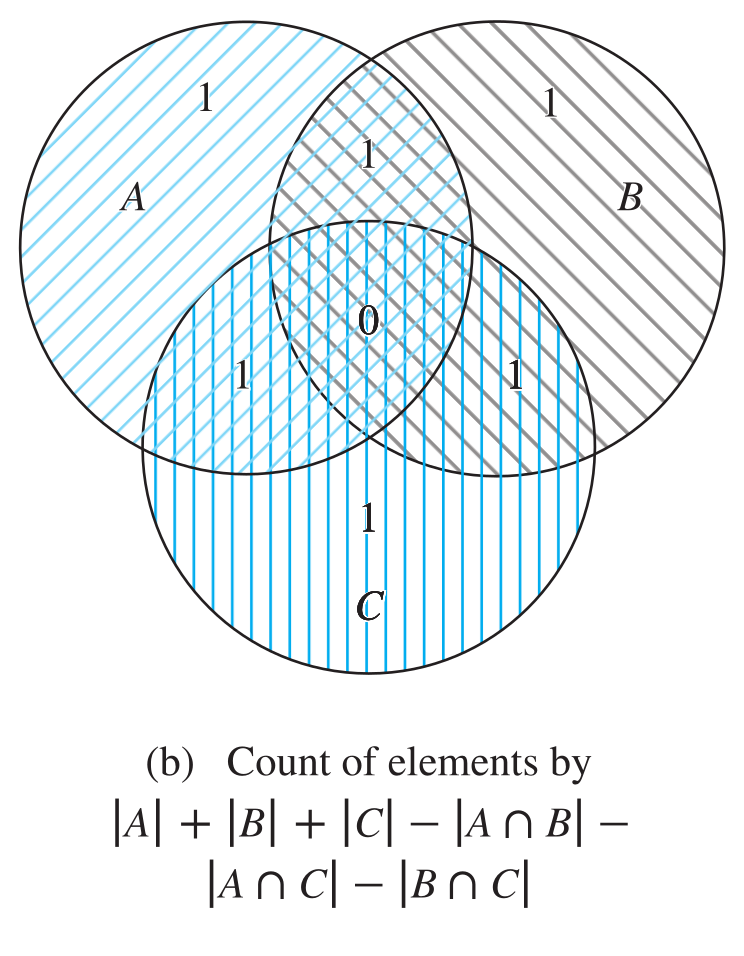
\includegraphics[scale=0.3]{81fig3b.png} 
\end{center}
\end{frame}

\begin{frame}{3. Sæt contd part 3}
   \begin{itemize}
       \item<1-> Hvad gør vi så? 
       \item<2-> Vi lægger $|A \cap B \cap C|$ til ligningen fra før.
   \end{itemize} 
\end{frame}

\begin{frame}{3. Sæt contd part 4}
\begin{center}
    
   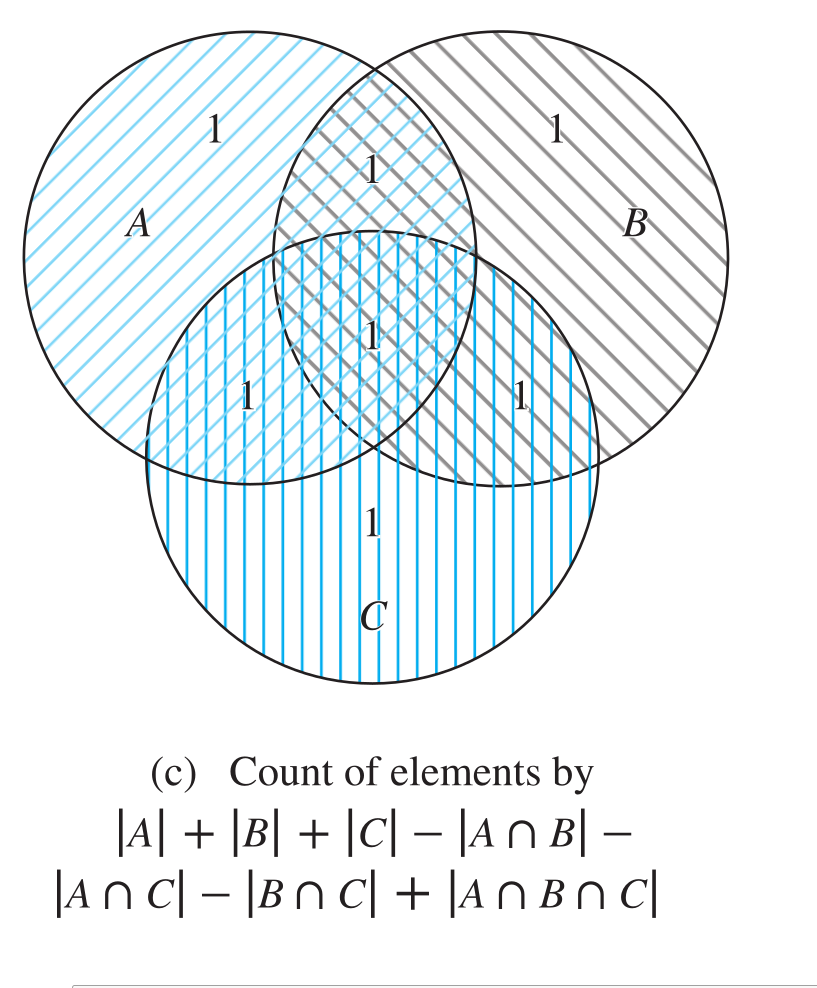
\includegraphics[scale=0.3]{81fig3c.png} 
\end{center}
\end{frame}
\begin{frame}{3. Sæt konklusion}
   \begin{itemize}
       \item Og på den måde har vi talt alle elementer præcis 1 gang!
   \end{itemize} 
\end{frame}

\begin{frame}[allowframebreaks]{Eksempel 4}
   \begin{itemize}
       \item Der er i alt 1232 studerende der har taget kurset "Spansk", 879 har taget "Fransk" og 114 har taget "Russisk". Ydermere har 103 taget kurser i både spansk og fransk, 23 i både spansk og russisk, og 14 i både fransk og russisk. Hvis 2092 studerende har taget mindst en af kurserne, hvor mange studerende har så taget et kursus i alle tre sprog? 
   \end{itemize} 
   
\end{frame}

\begin{frame}{Eksempel 4 part 2}

    \begin{itemize}
       \item<1-> Vi introducerer $S$ til at være antallet af studerende der har taget Spansk. $F$ fransk, og $R$ russisk. 
       \item<1-> $|S| = 1232, |F| = 879, |R| = 114, |S \cap F| = 103, |S \cap R| = 23, |F \cap R| = 14, |S \cup F \cup R| = 2092$.
       \item<2-> Vi sætter disse ind i ligningen: $$|S \cup F \cup R| = |S| + |F| + |R| - |S \cap F| - |S \cap R| - |F \cap R| + |S \cap F \cap R|$$
       \item<3-> Vi får: $$2092 = 1232 + 879 + 114 - 103 - 23 - 14 + |S \cap F \cap R|$$
       \item<4-> Til sidst løser vi for $|S \cap F \cap R| $ og finder at der er 7.
    \end{itemize}
\end{frame}

\begin{frame}{Eksempel 4 figur}
\begin{center}
    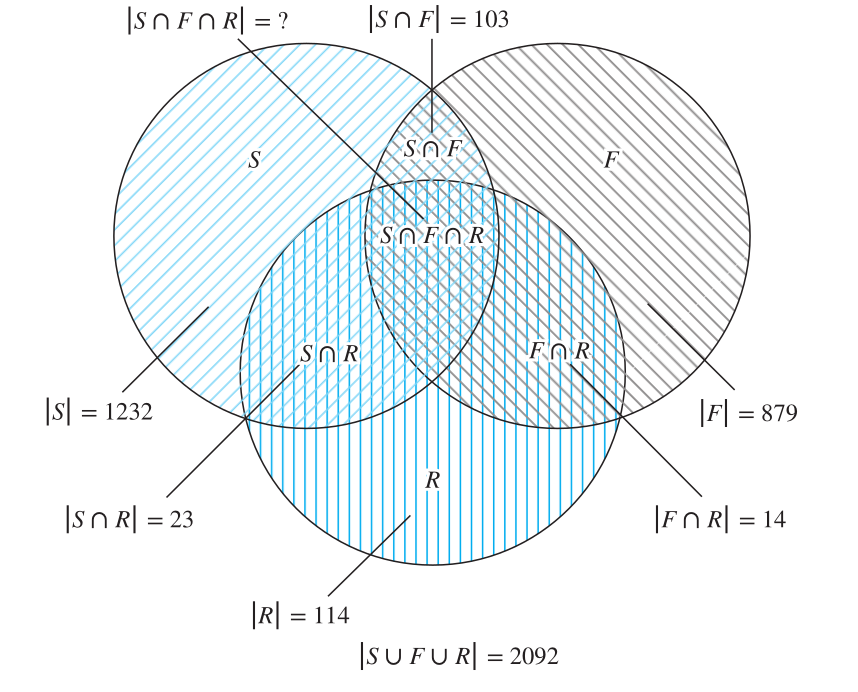
\includegraphics[scale=0.4]{81fig4.png}
\end{center}
\end{frame}

\begin{frame}{Generalisering}
   \begin{itemize}
       \item Hvordan generaliserer vi så, så fremfor 2 eller 3 sæt, at det er $n$ sæt (hvor $n$ er et positivt heltal)? 
   \end{itemize} 
\end{frame}

\begin{frame}{The Principle of Inclusion-Exclusion}
\begin{theorem}[THe Principle of Inclusion-Exclusion]
    
  Let $A_1, A_2, \ldots, A_n$   be finite sets. Then
  $$|A_1 \cup A_2 \cup \cdots \cup A_n| = \sum_{1 \leq i \leq n} |A_i| - \sum_{1 \leq i < j \leq n}|A_i \cap A_j| + \sum_{1 \leq i < j < k \leq n} |A_i \cap A_j \cap A-k|$$
  $$- \cdots + (-1)^{n+1} |A_1 \cap A_2 \cap \cdots \cap A_n|$$
\end{theorem}
\begin{itemize}
    \item<1-> Før vi kommer til beviset: Hvorfor tilføjer vi hvis antallet af sæt er ulige, men fjerner hvis det er lige? 
    \item<2-> Men tilføjer når det er lige, fordi der ellers bliver undertalt (undercounted)
    \item<2-> Men hvorfor fjerner man så? 
    \item<2-> Hvis $n$ er ulige, er elementerne først blevet talt én gang, så fjernet $\binom{n}{2}$ gange, tilføjet $\binom{n}{3}$ gange etc. Derfor må man til sidst fjerne intersection af alle sættene. 
\end{itemize}
\end{frame}

\begin{frame}{Theorem 1 Bevis}
\begin{proof}[Bevis part 1]
    Vi beviser formlen ved at vise at hvert element i fællesmængden bliver talt præcis en gang i højresiden af ligningen. 
    Antag at $a$ er et medlem af præcis $r$ af sættene $A_1, A_2, \ldots A_n$, hvor $1 \leq r \leq n$. Dette element bliver talt $C(r,1)$ gange af $\sum|A_i|$. Det bliver talt $C(r,2)$ gange af $\sum|A_i \cap A_j|$. Generelt set, bliver det talt $C(r,m)$  gange af summationen der har $m$ sæt af $A_i$. Derfor er dette element talt præcis
    $$C(r,1) - C(r,2) + C(r,3) - \cdots + (-1)^{r+1}C(r,r)$$
    gange af utdtrykket på højresiden af ligningen. 
\end{proof}
\end{frame}

\begin{frame}{Theorem 1 Bevis part 2}
\begin{proof}[Bevis part 2]
Vores mål er så at evaluere kvantiteten. Af corollary 2 i 6.4, har vi:
$$C(r,0) - C(r,1)+C(r,2)- \cdots + (-1)^rC(r,r) = 0$$
Dermed:
$$1 = C(r,0) = C(r,1) - C(r,2) + \cdots + (-1)^{r+1}C(r,r)$$
Derfor er hvert element i foreningsmængden talt præcis en gang af udtrykket i højresiden af ligningen. Dette beviser princippet af inclusion-exclusion.
\end{proof}
\begin{itemize}
    \item Vi ved at det er 1, fordi $c(r,0) - + - $etc = 1. Vi ved at $C(r,0) = 1$, og derfor må resten ($- C(r,1) + C(r,2)$ etc) være lig med 1, for at vi kan få 0.
\end{itemize}
\end{frame}

\begin{frame}{Corollary 2 6.4}
    \begin{corollary}[Corollary 2 Rosen 6.4]
    Let $n$ be a positive integer. Then
        $$\sum^n_{k=0} (-1)^k \binom{n}{k} = 0$$ 
    \end{corollary}
\end{frame}

\begin{frame}{Inclusion}
  \begin{itemize}
      \item<1-> Hvor mange led er der i inclusion-exclusion formlen? 
      \item<1-> Hint: Der er $n$ sæt. Husk tilbage til hvorfor vi tilføjer/fjerner sæt afhængigt af om $n$ er lige eller ulige. 
      \item<2-> Hint 2: Husk tilbage til corollary 1 i 6.4
      \item<3-> Corollary 1: Let $n$ be a nonnegative integer. Then $\sum^n_{k=0}\binom{n}{k} = 2^n$.
      \item<4-> Svar: $2^n - 1$. Siden vi ikke har $\binom{n}{0}$ med, som der er i Corollary 1, så fjerner vi 1.
  \end{itemize}  
\end{frame}

\begin{frame}{Reflektion}
   \begin{itemize}
       \item Hvad har sum og subtraction rule med inclusion-exclusion at gøre? 
       \item Hvad er corollary 1 fra 6.4?
       \item Hvad er corollary 2 fra 6.4? 
       \item Hvorfor tilføjer vi kun hvis det er et lige antal af sæt i ligningen? 
       \item Hvor mange led er der i teoremet? 
   \end{itemize} 
\end{frame}

\section{Applications of Inclusion-Exclusion}

\begin{frame}[allowframebreaks]{Alternativ Notation}
\begin{itemize}
    \item Der er en alterantiv notation der er nyttig i tælleproblemer
    \item Specifikt kan denne notation bruges til at løse problemer der spørger om antallet af elementer i et sæt der ikke har nogen af $n$ egenskaber, $P_1, P_2, \ldots, P_n$.
    \item Lad $A_i$ være subsettet der indeholder elementerne med egenskab $P_i$. Antallet af elementer med alle egenskaber $P_{i_1}, P_{i_2}, \ldots, P_{i_k}$ bliver noteret af $N(P_{i_1} \ldots P_{i_k})$. Altså:
    \item $|A_{i_1} \cap A_{i_2} \cap \cdots \cap A_{i_k}| = N(P_{i_1}P_{i_2} \ldots P_{i_k})$
   \item Hvis antallet af sæt med ingen af egenskaberne $P_1, P_2, \ldots, P_n$  er noteret som $N(P_1' P_2' \ldots P_n')$ of antallet af elementer i sættet er notered af $N$, følger det at: $$N(P_1'P_2' \ldots P_n') = N - |A_1 \cup A_2 \cup \cdots \cup A_n|$$.
   \item Vi ser fra inclusion-exclusion princippet at: $$N(P'_1 P'_2 \dots P'_n) = N - \sum_{1 \leq i \leq n} N(P_i) + \sum_{1 \leq i < j \leq n} N(P_i P_j)$$
   $$ - \sum_{1 \leq i < j < k \leq n} N(P_i P_j P_k) + \dots + (-1)^n N(P_1 P_2 \dots P_n). $$
   \item Spørgsmål: Hvorfor er det sidste led $(-1)^n \cdots$, og ikke $^{n+1}$?
\end{itemize}
\end{frame}

\begin{frame}{Eksempler}
   Tid til flere eksempler
   
\includegraphics[scale=0.4]{elmo.jpg}
\end{frame}

\begin{frame}{Eksempel 1}
   \begin{itemize}
        \item<1-> Hvor mange løsninger har $x_1 + x_2 + x_3 = 11$, hvor $x_1, x_2, x_3$ er ikke-negative heltal med $x_1 \leq 3, x_2 \leq 4, x_3 \leq 6$?
        (Til fremlægger: det næste punkt er et hint)
        \item<2-> Hint: Hvis en løsning har egenskaben $P_1$ hvis $x_1 > 3$, $P_2$ hvis $X_2 > 4$, $P_3$hvis $x_3 > 6$, hvor mange løsninger opfylder ulighederne? 
        \item<3-> $N(P'_1P'_2P'_3) = N - N(P_1) - N(P_2)-N(P_3) + N(P_1P_2) + N(P_1P_3)+N(P_2P_3) - N(P_1P_2P_3)$.
   \end{itemize} 
\end{frame}
\begin{frame}{Eksempel 1 ii}
   \begin{itemize}
        \item Hvor: 
        \item \( N \) = total number of solutions = \( C(3 + 11 - 1, 11) = 78 \),
        \item \( N(P_1) \) = (number of solutions with \( x_1 \geq 4 \)) = \( C(3 + 7 - 1, 7) = 36 \),
        \item \( N(P_2) \) = (number of solutions with \( x_2 \geq 5 \)) = \( C(3 + 6 - 1, 6) = 28 \),
        \item \( N(P_3) \) = (number of solutions with \( x_3 \geq 7 \)) = \( C(3 + 4 - 1, 4) = 15 \),
        \item \( N(P_1 P_2) \) = (number of solutions with \( x_1 \geq 4 \) and \( x_2 \geq 5 \)) = \( C(3 + 2 - 1, 2) = 6 \),
        \item \( N(P_1 P_3) \) = (number of solutions with \( x_1 \geq 4 \) and \( x_3 \geq 7 \)) = \( C(3 + 0 - 1, 0) = 1 \),
        \item \( N(P_2 P_3) \) = (number of solutions with \( x_2 \geq 5 \) and \( x_3 \geq 7 \)) = 0,
        \item \( N(P_1 P_2 P_3) \) = (number of solutions with \( x_1 \geq 4 \), \( x_2 \geq 5 \), and \( x_3 \geq 7 \)) = 0.
   \end{itemize} 
\end{frame}

\subsection{The Number of Onto Function}
\begin{frame}{Eksempel 2 i}
\begin{itemize}
    \item<1-> Hvor mange onto funktioner er der fra et sæt med 6 elementer til et sæt med 3 elementer? 
    \item<2-> Antag at elementer i codomainet er $b_1, b_2$ og $b_3$. Lad $P_1, P_2$ og $P_3$ være egenskaberne at $b_1,b_2$ og $b_3$ ikke er indenfor funktionens værdimængde. 
    \item<2-> Notér, at en funktion er onto hvis og kun hvis at den ikke har nogen af enskaberne $P_1P_2P_3$. Af inclusion-exclusion er antallet af funktioner:
    \item<2-> $$N(P_1'P_2'P_3')$$
    \item<2-> Hvor $N$ er det samlede antal af funktioner fra et sæt med 6 elementer til et med 3. 
\end{itemize}    
\end{frame}

\begin{frame}{Eksempel 2 ii}
   \begin{itemize}
    \item<1-> Det følger fra 6.1 at $N = 3^6$. Notér at $N(P_i)$ er antallet af funktioner der ikke har $b_i$ i sin værdimængde. Dermed i alt: 
    \item<2-> $3^6 - C(3,1)2^6 + C(3,2)1^6 = 729-192+3=540$
   \end{itemize} 
\end{frame}

\begin{frame}{Theorem 1}
   \begin{theorem}
       Let $m$ and $n$ be positive integers with $m \geq n$. Then, there are
       $$n^m - C(n,1)(n-1)^m+C(n,2)(n-2)^m- \cdots + (-1)^{n-1}C(n,n-1) \cdot 1^m$$
       onto functions from a set with $m$ elements to a set with $n$ elements. 
   \end{theorem} 
\end{frame}

\begin{frame}[allowframebreaks]{Onto functions og Stirling numbers}
   \begin{itemize}
       \item En onto funktion fra et sæt med $m$ elementer til et sæt med $n$ elementer svarer til en måde at distribuere $m$ elementer i definitionsmængden til $n$ bokse man ikke kan skelne imellem, sådan at ingen boks er tom, og så associér hver af de $n$ elementer fra værdimængden til en boks.
       \item Dette betyder at antallet af onto funktioner fra et sæt med $m$ elementer til et sæt med $n$ elementer er antallet af måder at distribuere $m$ objekter man kan skelne imellem til $n$ bokse man ikke kan skelne imellem, sådan at der ikke er nogen bokse der er tomme, ganget med antallet af permutationer af et sæt med $n$ elementer. (Phew)
       \item Dermed er antallet af onto funtkioner fra et sæt med $m$ elementer til et sæt med $n$ elementer lig med $n!S(m,n)$, hvor $S(m,n)$ er et \textit{Stirling number of the second kind}. 
   \end{itemize} 
\end{frame}

\begin{frame}{Eksempel 3}
   \begin{itemize}
       \item<1-> Hvor mange måder er der at tildele fem forskellige jobs til fire forskellige arbejdere hvis hver arbejder har mindst et job? 
       \item<1-> Hint: brug Theorem 1!
       \item<2-> Overvej tildelingen af jobs som en funktion fra sættet af fem jobs til sættet af fire arbejdere. 
       \item<3-> Dermed, fra theorem 1, er der: $$4^5 - C(4,1)3^5 + c(4,2)2^5-c(4,3)1^5=1024-975+192-4=240$$ måder at give hver arbejder mindst et job.
   \end{itemize} 
\end{frame}

\subsection{Derangements}

\begin{frame}{Eksempel 4: Hatcheck Problemet}
\begin{columns}
   \begin{column}{0.5\textwidth}
   \begin{itemize}
       \item  An ny medarbejder tjekker hattene af $n$ personer på en restaurant. Han glemmer dog at give numre til hver hat. Når kunderne kommer tilbage for at få deres hatter, giver tjekkeren en tilfældig hat fra sættet af de resterende hatte. Hvad er sandsynligheden at ingen får sin egen hat tilbage? 
   \end{itemize} 
   \end{column} 
   \begin{column}{0.5\textwidth}
        
\includegraphics[scale=0.5]{image.png}
   \end{column} 
\end{columns}
\end{frame}

\begin{frame}{Hatcheck ii}
   \begin{itemize}
       \item \textbf{Bemærk}: Svaret er antallet af måder hattene kan blive arrangeret på, så ingen hat er i sin originale position, divideret med $n!$. 
       \item En \textbf{derangement} er en permutation af objekter således at intet objekt er i sin originale position. For at løse dette problem må vi først finde ud af hvor mange af disse "derangements" der er i et sæt af $n$ objekter.
   \end{itemize} 
\end{frame}

\begin{frame}{Eksempel 5}
   \begin{itemize}
       \item Permutationen 21453 er en \textit{derangement} af 12345 fordi intet tal er tilbage i sin originale position. Dog er 21543 ikke en derangement af 12345 fordi permutationen har 4 i samme position. 
       \item Lad $D_n$ være antallet af derangements af $n$ objekter. For eksempel, $D_3 = 2$, fordi derangements af 123 er 231 og 312. 
   \end{itemize} 
\end{frame}

\begin{frame}{Theorem 2}
\begin{theorem}
    
       Antallet af derangements af et sæt med $n$ elementer er 
       $$D_n = n!\left [1 - \frac{1}{1!}  + \frac{1}{2!} - \frac{1}{3!} + \cdots + (-1)^n \frac{1}{n!}\right ]$$
\end{theorem}
\end{frame}


\begin{frame}{Theorem 2 Bevis}
   \begin{proof}
       Lad en permutation have egenskaben $P_i$ hvis det "fikser" element $i$ (altså lader det bliver på sin egen plads). Antallet af derangements er antallet af permutation der ikke har nogen af egenskaberne $P_i, i = 1, 2, \ldots, n$. Dette betyuder at $$D_n = N(P_1'P_2'\ldots P_n')$$.
       Ved brug af inclusion-exclusion, ved vi at: 
       $$D_n = N - \sum_i N(P_i) + \sum_{i < j} N(P_iP_j)$$
       $$- \sum_{i<j<k} N(P_iP_jP_k) + \cdots + (-1)^n N(P_1P_2 \ldots P_n)$$
       Hvor $N$ er antallet af permutationer af $n$ elementer. 
   \end{proof} 
\end{frame}

\begin{frame}{Theorem 2 Bevis ii}
   \begin{proof}
       Først, læg mærke til at $N = n!$. $N(P_i) = (n-1)!$. Vi får dette fra product rule, fordi $N(P_i)$ er antallet af permutationer som "fikser" element $i$, så den $i$'e position af permutationen er valgt, men hver af de resterende positioner kan blive fulgt som ønsket. Lignende, $$N(P_iP_j) = (n-2)!$$ fordi dette er tallet af permutationer som "fikser" (holder) elementerne $i$ og $j$, men hvor de andre $n-2$ elementer kan blive arangeret arbitrært. Generelt set, læg mærke til at: 
   \end{proof} 
\end{frame}

\begin{frame}{Theorem 2 Bevis iii}
   \begin{proof}
       $$N(P_{i_1}P_{i_2} \ldots P_{i_m}) = (n-m)!$$ fordi dette er antallet af permutations som holder elementerne $i_1, i_2, ..., i_m$, men hvor de andre $n-m$elementer kan blive arrangeret arbitrært. Fordi der er $C(n,m)$ måder at vælge $m$ elementer fra $n$, følger det at $$\sum_{1 \leq i \leq n} N(P_i) = C(n,1)(n-1)!$$
       
       $$\sum_{1 \leq i < j \leq n}N(P_iP_j) = C(n,2)(n-2)!$$
   \end{proof} 
\end{frame}

\begin{frame}{Theorem 2 Bevis iv}
   \begin{proof}
       Og generelt, 
       $$\sum_{1 \leq i_1 < i_2 < \cdots < i_m \leq n} N(P_{i_1}P_{i_2} \ldots P_{i_m}) = C(n,m)(n-m)!$$

       Konsekvent, hvis vi sætter disse ind i vores formel, får vi: 
       $$D_n = n! - C(n, 1)(n - 1)! + C(n, 2)(n - 2)! - \dots + (-1)^n C(n, n)(n - n)!$$
       $$= n! - \frac{n!}{1!(n - 1)!} + \frac{n!}{2!(n - 2)!} - \dots + (-1)^n \frac{n!}{n!0!}.$$
   \end{proof} 
\end{frame}

\begin{frame}{Theorem 2 Bevis v}
   \begin{proof}
   Vi simplicerer og får:
       $$D_n = n! \left[ 1 - \frac{1}{1!} + \frac{1}{2!} - \dots + (-1)^n \frac{1}{n!} \right].$$
   \end{proof} 
\end{frame}


\end{document}